\documentclass[12pt, a4paper]{report}
\usepackage[vmargin=20mm, hmargin=20mm]{geometry}
\usepackage[french]{babel}
\usepackage[T1]{fontenc}
\usepackage[utf8]{inputenc}
%\usepackage{ifthen}
%	\newboolean{isTelegram}
%	\setboolean{isTelegram}{true}
\usepackage{listings}
	\lstset{language=bash,%
	basicstyle=\small,%
	stringstyle=\ttfamily,%
	}
\usepackage{xcolor}
\usepackage[]{amsmath}
\usepackage[]{amsfonts}
\usepackage[]{amssymb}
	\everymath{\displaystyle}
\usepackage[]{float}
	\floatplacement{figure}{H}
	\floatplacement{table}{H}
\usepackage[]{graphicx}
	\setkeys{Gin}{width=0.7071\linewidth}
\usepackage[all,defaultlines=3]{nowidow}
\usepackage[]{hyperref}
	\hypersetup{
		colorlinks=true,
		linkcolor=blue,
		urlcolor=purple
	}
	\urlstyle{same}
\usepackage{ifthen}
	\newboolean{dyslexie}
	\setboolean{dyslexie}{false}
\ifthenelse{\boolean{dyslexie}}{% True
	\usepackage{arev}
	\setlength{\parskip}{1em}
	\renewcommand{\baselinestretch}{1.5}
	\usepackage[document]{ragged2e}
}{% False
	\usepackage{lmodern}
	\setlength{\parskip}{0.5em}
	\renewcommand{\baselinestretch}{1.25}
}
\title{Procédure rapide pour une debian \emph{Full Disk Encryption} sur un LVM chiffré sur un ordinateur en legacy/BIOS.}
\author{F.S. G.}
\date{Document créé le Samedi 15 Octobre 2022\\Version du \today{}.}
\setlength{\parskip}{0.5em}
\renewcommand{\baselinestretch}{1.25}
\begin{document}
\maketitle

%\begin{abstract}
Ce document traite d'une installation non conventionnelle d'une distribution debian GNU/Linux sur un ordinateur en mode Legacy/BIOS, une partie dédiée à l'installation avec uefi est disponible à la section \ref{sec-uefi-machine}.

Ce document reprend chronologiquement les commandes saisies lors de l'installation dans une machine virtuelle et les fichiers de configuration.
%\end{abstract}

\chapter*{Préambule et indications}
\addcontentsline{toc}{chapter}{Préambule et indications}
Depuis ma découverte, il y a quelques années de la capacité de chiffrement des distributions linux, réglant outre un problème de confidentialité niveau matériel, celui aussi de la confidentialité dans de nombreuses occasions~; la recherche de la configuration avancée la plus adaptée à mes besoins de sécurité m'a semblé être un point crucial à aborder dans tout système utilisé.

Passant d'aucune partition chiffrée à deux partitions (\emph{swap} et \texttt{/home}) puis ensuite à trois partitions chiffrées (\texttt{/}, \texttt{/home} et \emph{swap}) pour finir par avoir tout le système sauf le dossier \texttt{/boot} dans une partition unique, dans un LVM\footnote{L.V.M.~: Logical Volume Management \url{https://fr.wikipedia.org/wiki/Gestion_par_volumes_logiques}.} sur un chiffrement, j'ai alors découvert avec la distribution archlinux que tout pouvait être dans la partition protégée, quand je dis tout, je fais référence à \texttt{/boot} compris.

C'est alors devenu la recherche d'une solution pour l'autre distribution que j'affectionne énormément~: j'ai nommé debian.

Par défaut, l'installateur officiel debian refuse que le dossier \texttt{/boot} soit chiffré, y compris en passant par l'entrée Expert proposée au démarrage. 
Ce document répond à cette question presque \emph{métaphysique}~: quelle procédure suivre pour procéder à cette installation en mode \emph{full disk encryption}~?

Évidement, cher lecteur ou chère lectrice, la solution évidente est de sortir de l'installation conventionnelle pour se lancer dans une installation très proche de celle d'archlinux ou de gentoo\footnote{Gentoo est une distribution où l'installation se fait manuellement en suivant un guide et l'installation ou la mise à jour des logiciels se fait par la compilation du code source par défaut.}, à la main, presque à l'ancienne, avec de la bonne ligne de commande à souhait et une procédure à suivre dans l'ordre permettant aux modules idoines de trouver leur place dans les fichiers de configuration.

Cette sortie du protocole standard d'installation permet une accaparation du processus traditionnel, j'y vois également intérêt salvateur en cas de réinstallation du système~: en effet lors d'une réinstallation d'une distribution debian utilisant l'installateur officiel dans une configuration de type partitions dans un lvm dans un conteneur chiffré, tout est détruit. 
Certains dans différents salons m'exprimaient leur désintérêt de cette procédure par rapport à une installation où les trois partitions existent déjà et sont chiffrées indépendamment (la racine, le swap et le home), j'arguais que plusieurs chiffrement m'ont montré une utilisation plus intense du processeur, je devrai cependant vérifier à nouveau ceci.

C'est ainsi que par le passé j'ai passé plusieurs heures, ordinateur allumé, pendant la nuit, pour sauvegarder les données entre un vieux disque en stressant pour qu'il ne lâche pas et son transfert vers un support temporaire puis une réinstallation complète puis encore plusieurs heures pour recopier le contenu depuis le support externe temporaire vers la nouvelle installation toute fraîche. 
La connaissance plus fine du processus d'installation permettra justement d'éviter cet écueil et de pouvoir effectuer une restauration du système en cas de crash important.

Avant de commencer je vais poser quelques prérequis d'exécution pour que tout fonctionne proprement. 
Dans un premier temps il est nécessaire de comprendre que l'installation ayant été effectuée dans une machine virtuelle de type VirtualBox, beaucoup de problèmes matériels sont \emph{de facto} éludés.

Plus de renseignements sur la distribution debian sont disponibles~:
\begin{itemize}
	\item \url{https://fr.wikipedia.org/wiki/Debian}
	\item \url{https://www.debian.org/}
	\item \url{https://www.infothema.fr/forum/index.php?topic=7.0} et plus précisément l'image suivante~:\newline \url{http://www.infothema.fr/documents/juillet-2012/750_infographic_debian_history-fr-v08.png}
\end{itemize}

\paragraph{Ressources externes.}
%Une autre information dont il faut tenir compte, les liens. 
Dans la compilation actuelle du document, les liens internes sont en bleu, les liens vers des ressources externes -- sur internet -- sont quant à eux en pourpre.

\paragraph{Convention typographique du code.} 
Afin de faciliter la visualisation du code et des commandes à saisir, celles-ci sont encadrées par des lignes horizontales et la police de caractère de toute commande et \emph{in extenso} de tout programme à exécuter sera en police à chasse fixe. 
L'exemple qui suit montre par exemple un exemple de commande \texttt{echo}~:

\noindent\rule{\linewidth}{0.5pt}
\begin{verbatim}
anonymous@Bore:~$ echo "Mon petit cheval trotte."
Mon petit cheval trotte.
\end{verbatim}
\rule{\linewidth}{0.5pt}

\paragraph{Utilisateur et super-utilisateur.}
Je rappelle que par convention l'information affichée au début d'une ligne de terminal est appelée le \emph{prompt\/} et que celle-ci permet d'avoir de multiples informations. 
La plus importante se trouve à la fin du prompt~:
\begin{itemize}
	\item si le prompt finit par le symbole \texttt{\$} cela signifie que le compte actif est celui d'un utilisateur normal, sauf spécificité,
	\item si le prompt finit par le symbole \texttt{\#} c'est que la commande qui sera saisie se fera avec les privilèges de l'administrateur.
\end{itemize}

\chapter{Dans le host debian-live}
La première partie des commandes s'effectue dans l'environnement live de debian. 
Pourquoi~? 
Tout simplement parce que cet environnement contient déjà les commandes permettant de préparer le support du futur système et le futur système.

Je suppose que l'installation se fait par un câble ethernet directement relié à la box avant démarrage ou à tout système permettant l'attribution automatique des paramètres réseaux, ce choix est basé sur la facilité de l'établissement d'une connexion internet avec un tel dispositif, la commande de connexion étant tout simplement \texttt{dhcpcd} ou \texttt{dhclient} si l'interface n'est pas déjà configurée au moment du démarrage et dans un deuxième temps rien ne dit que le système \emph{live} debian sur lequel est initiée cette installation reconnaîtra la carte wifi. 
Qui plus est, la connexion filaire est plus stable ce qui sera pratique pour la grosse quantité de données.

\noindent\rule{\linewidth}{0.5pt}
\begin{verbatim}
[anonymous@Pl4t1n3 Temp2Push]$ ip addr
1: lo: <LOOPBACK,UP,LOWER_UP> mtu 65536 qdisc noqueue state UNKNOWN group \
	default qlen 1000
    link/loopback 00:00:00:00:00:00 brd 00:00:00:00:00:00
    inet 127.0.0.1/8 scope host lo
       valid_lft forever preferred_lft forever
    inet6 ::1/128 scope host 
       valid_lft forever preferred_lft forever
2: enp4s0: <BROADCAST,MULTICAST,UP,LOWER_UP> mtu 1500 qdisc mq state UP group \
	default qlen 1000
    link/ether 70:85:c2:0d:03:1c brd ff:ff:ff:ff:ff:ff
    inet 192.168.1.31/24 brd 192.168.1.255 scope global dynamic noprefixroute \
    enp4s0
       valid_lft 85948sec preferred_lft 75148sec
    inet6 fe80::9fdd:8803:dc38:c07d/64 scope link 
       valid_lft forever preferred_lft forever
[anonymous@Pl4t1n3 Temp2Push]$
\end{verbatim}
\rule{\linewidth}{0.5pt}

La commande \texttt{ip addr} précédente montre sur un deuxième ordinateur le résultat de sa sortie --~la carte ethernet n'est pas la même que dans le système live dont la sortie est montré plus loin~--, il est très complet, voire trop, et peut dérouter un peu un utilisateur non habitué aux lignes de commandes, mais elle permet d'afficher les détails de toutes les cartes reconnues, la commande \texttt{networkctl status} donne aussi les informations de toute carte configurée, avec moins de détails mais du coup plus de lisibilité.

Dans mon cas sur le système live démarré dans la virtualbox, j'obtiens les lignes suivantes --~la carte réseau étant cette fois-ci enp0s3 dans la virtualbox et non enp4s0 comme dans le deuxième ordinateur~:

\noindent\rule{\linewidth}{0.5pt}
\begin{verbatim}
root@debian:~# networkctl status
WARNING: systemd-networkd is not running, output will be incomplete.

*        State: n/a
  Online state: unknown
       Address: 10.0.2.15 on enp0s3
               fe80::1c29:8137:2499:ad5b on enp0s3
       Gateway: 10.0.2.2 on enp0s3
root@debian:~#
\end{verbatim}
\rule{\linewidth}{0.5pt}

Les images de systèmes \emph{live} de debian se trouvent dans la page \url{https://cdimage.debian.org/cdimage/} et regroupent aussi d'autres types d'images dont les images avec firmware que je ne saurais que recommander dans le cas de matériel exotique.

Une fois l'image gravée, il suffit de démarrer dessus avec les touches \fbox{F2}, \fbox{F10} ou encore \fbox{F9} ou encore \fbox{F12}.

\section{Mise à jour de la base des paquets et installation des outils}

Lors de la future installation et la préparation du support il est nécessaire d'avoir quelques outils, \texttt{wget} pour récupérer les paquets depuis internet, \texttt{debootstrap} pour installer le système de base, et comme l'installation présentée ici se base sur un lvm chiffré, il faut les outils habituels permettant leur manipulation, respectivement \texttt{lvm2} et \texttt{cryptsetup} 

\noindent \rule{\linewidth}{0.5pt}
\begin{verbatim}
apt update
apt install wget debootstrap lvm2 cryptsetup
cryptsetup benchmark
\end{verbatim}
\rule{\linewidth}{0.5pt}

Afin de tester quels sont les chiffrement et déchiffrement les plus rapides ou optimaux suivant le matériel, j'exécute la commande~:\newline
\begin{verbatim}
cryptsetup benchmark
\end{verbatim}

Une fois cela effectué je note ces paramètres de côté pour la suite.

\section{Préparation du support cible (futur système)}
Je vais supposer que mon disque futur d'installation est un disque neuf, sans aucune table de partitions créées et sur une machine de type \emph{Legacy} BIOS / BIOS.

\begin{figure}
	\centering
	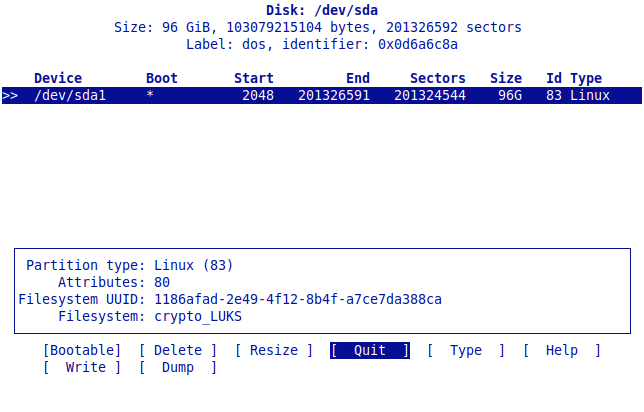
\includegraphics{cfdisk.png}
	\caption{L'interface rudimentaire mais compréhensible de cfdisk.}
\end{figure}

D'abord on commence par charger la commande \texttt{fdisk} ou tout autre outil de partitionnement, par exemple \texttt{cfdisk}.

\noindent \rule{\linewidth}{0.5pt}
\begin{verbatim}
fdisk /dev/sda
\end{verbatim}
\rule{\linewidth}{0.5pt}

Ma préférence va vers \texttt{fdisk} car il est plus rustique, on ne se refait pas, et également car contrairement à \texttt{cfdisk} qui fonctionne très bien pour le formatage de partitions sur un disque possédant déjà une table de partitions, \texttt{fdisk} quant à lui permet aussi de générer une nouvelle table de partitions. 
Je vais donc~:
\begin{itemize}
	\item Créer une nouvelle table de partitions de type \texttt{msdos} (BIOS)~: \fbox{o} 
	\item Une nouvelle partition \fbox{n} 
	\item De type primaire \fbox{p}
	\item on garde le numéro par défaut assigné (\textbf{1}) : \fbox{enter} 
	\item Qui démarre à l'\emph{offset} par défaut \fbox{enter} 
	\item Avec la taille par défaut \fbox{enter} 
	\item Ensuite on marque la seule partition existante comme démarrable (\emph{flag bootable}) \fbox{a} 
	\item Puis on écrit cette nouvelle table de partitionnement et synchronisation du disque \fbox{w}
\end{itemize}

\begin{figure}
	\centering
	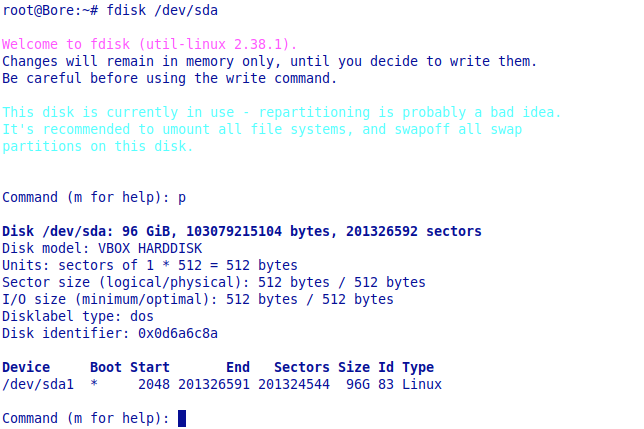
\includegraphics{fdisk.png}
	\caption{L'interface ultrarudimentaire de fdisk.}
\end{figure}

Comme il n'y a qu'une seule partition, on la formate de suite en réutilisant les paramètres notés auparavant~:

\noindent \rule{\linewidth}{0.5pt}
\begin{verbatim}
cryptsetup lukfFormat -y -v --cipher=(aes-xts-plain64) \
   --hash=(sha256) --key-size=(256) --type=luks1 /dev/sda1
\end{verbatim}
\rule{\linewidth}{0.5pt}

Puis l'ouverture de la partition chiffrée sous le nom de volume ```\$namevolume''.

\noindent \rule{\linewidth}{0.5pt}
\begin{verbatim}
cryptsetup luksOpen /dev/sda1 $namevolume
\end{verbatim}
\rule{\linewidth}{0.5pt}

Vient ensuite la création du lvm dans \$namevolume et des différentes partitions~:

\noindent \rule{\linewidth}{0.5pt}
\begin{verbatim}
pvcreate /dev/mapper/$namevolume
vgcreate $monvg /dev/mapper/$namevolume
lvcreate $monvg -L 42G -n Racine
lvcreate $monvg -L 8G -n Memoire
lvcreate $monvg -l +100%FREE -n Utilisateurs
\end{verbatim}
\rule{\linewidth}{0.5pt}

\begin{itemize}
	\item \texttt{pvcreate} crée le lvm dans la partition chiffrée \texttt{/dev/mapper/\${}namevolume}
	\item \texttt{vgcreate} crée un groupe de volume dans le lvm dans la partition chiffrée \ldots
	\item \texttt{lvcreate} crée un volume chiffré dans le groupe de volumes dans le lvm dans la partition chiffrée
	\item \texttt{-L} fixe la taille du volume \texttt{-n} lui attribut un nom
	\item \texttt{-l +100\%{}FREE} attribue tout l'espace restant dans le groupe de volume créé par cette commande.
\end{itemize}

Comme précédemment un nom générique sera donné au groupe de volume, à savoir ``\texttt{\${}monvg}'', et pour les noms de partition j'ai simplement utilisé leur futur rôle, ``\texttt{Racine}'' accueillera la future racine du système, ``\texttt{Memoire}'' sera le \emph{swap} \emph{i.e.\/} la future mémoire additionnelle et ``\texttt{Utilisateurs}'' sera la partition dédiée à l'hébergement des données des utilisateurs.
On passe par l'étape formatage de chaque partition nouvellement créée~:

\noindent \rule{\linewidth}{0.5pt}
\begin{verbatim}
mkfs.ext4 /dev/$monvg/Racine
mkswap /dev/$monvg/Memoire
mkfs.ext4 /dev/$monvg/Utilisateurs
\end{verbatim}
\rule{\linewidth}{0.5pt}

Puis le montage de ces partitions~:

\noindent \rule{\linewidth}{0.5pt}
\begin{verbatim}
mkdir /mnt
mount /dev/$monvg/Racine /mnt
swapon /dev/$monvg/Memoire
mkdir /mnt/home
mount /dev/$monvg/Utilisateurs /mnt/home
\end{verbatim}
\rule{\linewidth}{0.5pt}

\texttt{\$namevolume} et \texttt{\$monvg} sont évidemment à changer en fonction du souhait de chaque personne évidemment, par exemple je vais utiliser B (Bore) et 5 (son numéro atomique) respectivement dans mon installation dont le résultat final sera montré à la fin du document..

\section{Installation du système de base dans le dossier cible}
Pour l'installation du système je choisis la distribution actuelle stable, nom de code \emph{bullseye} qui sera suffisante pour ce système de test. Mais bien sûr, dans le cas d'un matériel récent, je ne saurai que recommander la future debian 12 dont le nom de code est \emph{bookworm}.

Tout commence par l'installation d'un système de base récupéré sur le site de debian, je choisis le site français, je fixe l'architecture de la future installation, pour ce processeur 64~bits (\texttt{amd64}) la distribution bullseye et le chemin vers la future racine actuellement montée dans le dossier \texttt{/mnt}.

\noindent \rule{\linewidth}{0.5pt}
\begin{verbatim}
debootstrap --arch=amd64 bullseye /mnt http://ftp.fr.debian.org/debian/
\end{verbatim}
\rule{\linewidth}{0.5pt}

Cette commande a de particulier que l'ordre des paramètres est important, plusieurs essais infructueux ont été essuyés parce que l'ordre n'était pas celui-là.
Si vous souhaitez installer la future version actuellement disponible dans les dépôts, son nom de code est \emph{bookworm\/}.

\section{Préparation du changement de racine}
La racine est actuellement sur le système \emph{live}, il faut passer sur la nouvelle racine actuellement attachée sur \texttt{/mnt} afin de configurer le futur système et ajouter des paquets additionnels avant le redémarrage, cette opération s'effectue par la commande \texttt{chroot} (\emph{change root}), cependant pour que le passage permette quand même le fonctionnement du système il est nécessaire de copier le fichier de résolution des noms de sites web puisque nous allons télécharger depuis internet tous les paquets additionnelles (\texttt{/etc/resolv.conf}), ensuite la racine temporaire doit communiquer avec le matériel, donc les dossiers\footnote{ici plutôt les \emph{nodes}} dans \texttt{/dev}, \texttt{/proc} et \texttt{/sys} doivent être temporairement reliés à ceux de la future racine, respectivement \texttt{/mnt/dev}, \texttt{/mnt/proc} et \texttt{/mnt/sys}~:

\noindent \rule{\linewidth}{0.5pt}
\begin{verbatim}
cp -v /etc/resolv.conf /mnt/etc/resolv.conf
mount --rbind /dev /mnt/dev
mount --make-rslave /mnt/dev
mount --rbind /sys /mnt/sys
mount --make-rslave /mnt/sys
mount --rbind /proc /mnt/proc
mount --make-rslave /mnt/proc
chroot /mnt /bin/bash
\end{verbatim}
\rule{\linewidth}{0.5pt}

La dernière commande de cette série effectue le changement de racine dans le dossier les paramètres indiquent la nouvelle racine en premier /mnt --~qui devient désormais \texttt{/}~-- et ensuite où se trouve l'interpréteur de commande --~\emph{shell}~-- dans la nouvelle racine.

\chapter{Dans le chroot}

Désormais dans la future racine devenue nouvelle racine temporaire, il est temps de commencer la configuration du futur système, configuration qui sera basique pour laisser ensuite le temps d'installer les paquets en fonction des besoins.

\section{Mot de passe de root}
L'une des premières actions à réaliser consiste pour moi à créer un mot de passe pour root, l'administrateur. 
C'est le rôle de cette commande~:

\noindent \rule{\linewidth}{0.5pt}
\begin{verbatim}
passwd root
\end{verbatim}
\rule{\linewidth}{0.5pt}

\section{Édition du fichier \texttt{/etc/apt/sources.list}}
Ici va être configuré dans le nouvel environnement le fichier \texttt{sources.list} qui contient la liste des dépôts. 
J'utilise l'éditeur \texttt{nano} pour éditer le fichier, il en existe pléthore~: \texttt{vi}, \texttt{emac}, \texttt{ed}, \texttt{nedit}, \ldots

\noindent \rule{\linewidth}{0.5pt}
\begin{verbatim}
nano -w /etc/apt/sources.list
\end{verbatim}
\rule{\linewidth}{0.5pt}

\paragraph{Un exemple de fichier.} 
Voici typiquement le type de fichier que je vais saisir, il est minimaliste mais suffisant pour cette machine~:

\noindent \rule{\linewidth}{0.5pt}
\begin{verbatim}
# dépot principal de debian
deb http://ftp.fr.debian.org/debian/ bullseye main contrib non-free

# Updates disponibles
deb http://ftp.fr.debian.org/debian/ bullseye-updates main contrib non-free
deb http://ftp.fr.debian.org/debian/ bullseye-proposed-updates main contrib non-free

# paquets de la version n+1 de debian compatibles avec la version n
deb http://ftp.fr.debian.org/debian/ bullseye-backports main contrib non-free

# mises à jour de sécurité
deb http://ftp.fr.debian.org/debian-security/ bullseye-security main contrib non-free
\end{verbatim}
\rule{\linewidth}{0.5pt}

Plus d'informations sont disponibles sur \href{https://wiki.debian.org/fr/SourcesList}{le wiki de debian} le wiki officiel du projet debian.

Une fois le fichier sources rempli, il s'agit de mettre à jour la liste des paquets disponibles et d'installer de quoi configurer le fuseau horaire et les locales --~paramètres linguistiques locaux~:

\noindent \rule{\linewidth}{0.5pt}
\begin{verbatim}
apt update
apt install locales console-setup
dpkg-reconfigure locales
dpkg-reconfigure tzdata
dpkg-reconfigure console-setup
\end{verbatim}
\rule{\linewidth}{0.5pt}

\paragraph{Notez bien.} \texttt{dpkg-reconfigure} permet de configurer les paramètres pour chaque paquet installé. 
Je présume évidemment que le lecteur ou la lectrice de ce document sera pleinement familiarisé(e) avec le concept de paquet. Si c'est le cas passez à la section \ref{subsec-crypttab-fstab} sinon allez lire la section \ref{subsec-install-progs-linux}.

\section{Les fichiers \texttt{/etc/fstab} et \texttt{/etc/crypttab}} \label{subsec-crypttab-fstab}
Afin de ne pas avoir à recopier l'intégralité de l'UUID de la partition \texttt{/dev/sda1} je vais ajouter par la commande \texttt{blkid} cette information dans le fichier \texttt{/etc/crypttab}.

\noindent \rule{\linewidth}{0.5pt}
\begin{verbatim}
blkid -o value -s UUID /dev/sda1 >> /etc/crypttab
nano -w /etc/crypttab
\end{verbatim}
\rule{\linewidth}{0.5pt}

Pourquoi l'UUID~? Si un jour pour une raison x ou y le disque change d'ordre (et devient \texttt{/dev/sdb} par exemple) le système ne pourra pas démarrer, alors que l'UUID ne change qu'au formatage de la partition.

Le fichier \texttt{/etc/crypttab} doit ressembler peu ou prou à ce celui reproduit dans la ligne suivante, sachez qu'il peut y avoir une ligne de commentaire expliquant les premiers champs, mais ça n'est pas une obligation.

\noindent \rule{\linewidth}{0.5pt}
\begin{verbatim}
$namevolume	UUID=(uuid de /dev/sda1)		none		luks
\end{verbatim}
\rule{\linewidth}{0.5pt}

\paragraph{Notez.} D'autres options peuvent être ajoutées au dernier paramètre, par exemple ``discard'' qui paraît être déconseillée pour les disques ssd.

Je peux faire de même avec les partitions incluses dans le LVM en incluant toutes les informations dans le fichier \texttt{/dev/fstab}.

\noindent \rule{\linewidth}{0.5pt}
\begin{verbatim}
blkid /dev/mapper/$monvg- >> /etc/fstab
nano -w /etc/fstab
\end{verbatim}
\rule{\linewidth}{0.5pt}

Une fois dans le fichier \texttt{/etc/fstab} via l'utilisation de l'éditeur de textes préféré, il suffit d'ajouter les lignes pour déclarer chaque partition. 
Le fait d'avoir ajouté précédemment via la commande \texttt{blkid} les lignes relatives aux partitions permet de savoir à quelle partition correspond chaque volume logique.

La dénomination peut être changée, au choix on peut utiliser \texttt{/dev/mapper/\${}monvg-Racine} ou bien \texttt{/dev/\${}monvg/Racine}, je choisis par commodité la seconde forme d'écriture.

\noindent \rule{\linewidth}{0.5pt}
\begin{verbatim}
# ligne correspondante a /dev/mapper/$monvg-Racine
/dev/$monvg/Racine	 /	 ext4		rw,errors=remount-ro		0	1
# ligne correspondante a /dev/mapper/$monvg-Memoire
/dev/$monvg/Memoire	 swap		swap		sw	0	0
# ligne correspondante a /dev/mapper/$monvg-Utilisateurs
/dev/$monvg/Utilisateurs 	/home	ext	4	defaults		0	2
\end{verbatim}
\rule{\linewidth}{0.5pt}

\section{Installation du futur système}

Installation de la configuration minimaliste qui sera la base du futur système. 
Le symbole \og{}~\textbackslash{}~\fg{} indique que la commande n'est pas finie sur la même ligne dans le terminal mais que pour des raisons de présentation de ce document, cette suite a été mise à la ligne suivante.

La liste des paquets précédents permet d'avoir un système opérationnel avec une interface minimaliste. 
Si vous souhaitez d'autres interfaces graphiques installées plus ou moins automatiquement ou la configuration de la langue, effectuez la recherche suivante et notez les noms des paquets qui vous intéressent.

\noindent \rule{\linewidth}{0.5pt}
\begin{verbatim}
apt-cache search task-
\end{verbatim}
\rule{\linewidth}{0.5pt}

Dans mon cas je vais procéder à une installation d'une base minimale de paquets suffisante pour redémarrer en mode textuel, puis une fois le redémarrage effectué j'installerai les paquets nécessaires et obtiendrai du coup le système opérationnel. 
Je rappelle ici que j'ai choisi de ne pas utiliser la connexion wifi pour l'installation et qu'au redémarrage évidemment je ne pense pas encore l'utiliser, d'où l'absence de paquets tels que \texttt{wpasupplicant}, \texttt{network-manager} et \texttt{network-manager-gnome} pour gérer les connexions, de même aucun firmware n'est installé à ce stade bien que je puisse les lister par la commande \texttt{lspci} puis installer le firmware adéquat en cherchant le résultat de la sortie de cette commande.

\noindent \rule{\linewidth}{0.5pt}
\begin{verbatim}
apt update
apt install linux-image-amd64 dhcpcd5 cryptsetup lvm2 grub2 dialog sudo
\end{verbatim}
\rule{\linewidth}{0.5pt}

Afin que l'intégralité des paquets soient visibles, j'ai séparé la commande d'installation des paquets en plusieurs lignes. 
Notez que je choisis le paquet \texttt{dhcpcd5} au lieu de l'habituel \texttt{dhclient}. 
Le paquet \texttt{linux-image-amd64} est un métapaquet qui permettra par la suite de laisser le noyau évoluer dans le temps. 
Son nom est également plus simple.

L'installation de locales et de tzdata n'est pas nécessaire puisque faite auparavant, quant à sudo il va être indispensable par la suite puisque j'envisage avant de quitter le système temporaire de créer un utilisateur courant et de l'inscrire au groupe sudo.

\section{Configuration de Grub et et génération de l'InitRamFS}

Ici vont être configurés puis générés grub et l'initramfs. 
Comme la précaution a été prise de générer et modifier tous les fichiers critiques que sont \texttt{/etc/crypttab} et \texttt{/etc/fstab} la génération des fichiers de configuration va détecter cette installation particulière et charger tout le nécessaire pour assurer un redémarrage.

Attention cependant, le fichier \texttt{/etc/default/grub} n'a pas été modifié avec la ligne indispensable pour indiquer que le disque système est entièrement chiffré, incluant le dossier primordial \texttt{/boot}. 
C'est pour cette raison que la partition chiffrée par \texttt{cryptsetup} l'a été avec le paramètre \texttt{\-\-type=luks1} sans quoi \texttt{grub} sera incapable de l'ouvrir à l'heure actuelle.
Aussi le paramètre \texttt{GRUB\_ENABLE\_CRYPTODISK=y} (en respectant la casse) est {\bf indispensable}~!

\noindent \rule{\linewidth}{0.5pt}
\begin{verbatim}
echo "GRUB_ENABLE_CRYPTODISK=y" >> /etc/default/grub
blkid -o value -s UUID /dev/sda1 >> /etc/default/grub
nano -w /etc/default/grub
\end{verbatim}
\rule{\linewidth}{0.5pt}

Une fois ces deux ajouts effectués, le fichier doit être modifié légèrement~:
\begin{verbatim}
GRUB_CMDLINE_LINUX="cryptdevice=UUID=(l'uuid de sda1):$namevolume"
\end{verbatim}
Il est possible également de changer le paramètre de la ligne \newline 
\texttt{GRUB\_CMD\_LINUX\_DEFAULT="quiet"} en supprimant le mot quiet. 
Reste alors la configuration finale du noyau et de grub.

\noindent \rule{\linewidth}{0.5pt}
\begin{verbatim}
update-initramfs -u
grub-install /dev/sda
update-grub2
\end{verbatim}
\rule{\linewidth}{0.5pt}

Grub est le programme que je choisis --~il en existe d'autres~-- pour démarrer le système, quant à l'initramfs il s'agit d'une image minimaliste de linux qui est lue et chargée en mémoire au démarrage pour permettre la vérification du système racine\footnote{dans notre cas le déchiffrement de la partition, le chargement du lvm et le montage de la racine dans ce lvm chiffré} puis de laisser la main au vrai système après vérification de la racine.

Je choisis évidemment la version grub2 qui est plus récente et permet une configuration plus fine. 
Il existe d'autres chargeurs de démarrage tels que lilo ou encore refind que je n'exploite pas vraiment.

\section{Ajout du nouvel utilisateur et inscription au groupe des administrateurs \texttt{sudo}}
Il suffit désormais d'ajouter l'utilisateur courant et si besoin de l'ajouter également au groupe d'utilisateurs administrateurs (sudo).

\noindent \rule{\linewidth}{0.5pt}
\begin{verbatim}
adduser $nouvelutilisateur
adduser $nouvelutilisateur sudo
\end{verbatim}
\rule{\linewidth}{0.5pt}

L'utilisateur étant configuré, il va falloir désormais quitter l'installation ou procéder à d'autres ajouts de paquets avant de quitter.

\section{Ajout d'autres paquets.}
Si vous souhaitez installer une interface graphique, d'autres paquets, c'est bien sûr ici qu'il faut le faire.

\section{Sortie de l'environnement temporaire \texttt{chroot}}
Cette sortie s'effectue simplement par la commande \texttt{exit} et le prompt devrait sans doute changer aussi au passage.

\noindent \rule{\linewidth}{0.5pt}
\begin{verbatim}
exit
\end{verbatim}
\rule{\linewidth}{0.5pt}

\section{Redémarrage de la machine pour accéder au nouveau système}
Une fois de retour dans le \emph{live} de debian, un reboot suffira à démonter tous les volumes logiques, tous les groupes de volumes et les partitions chiffrées.

\noindent \rule{\linewidth}{0.5pt}
\begin{verbatim}
reboot
\end{verbatim}
\rule{\linewidth}{0.5pt}

\chapter{Au démarrage}
Lors des démarrages il faudra porter son attention sur les particularités suivantes~:
\begin{itemize}
	\item lors de la première phase de démarrage, le micronoyau demandera un mot de passe, à ce moment-là le clavier est en \bsc{qwerty}, les ponctuations ne sont pas au même endroit, certaines lettres aussi, il faudra donc avoir une image de clavier \bsc{qwerty} les premières fois pour repérer les positions des touches correspondant au mot de passe du volume chiffré à l'installation,
	\item la moindre erreur dans la saisie du mot de passe, ou si vous ne pressez pas sur la touche de retour arrière le nombre exact de touches à corrriger dans le cas où vous auriez vu que vous vous êtes trompé, génèrera un message d'erreur, donc l'arrêt illico du démarrage,
	\item une fois la phase de démarrage (écran grub) démarrée, le clavier passera en français, donc il se peut que certaines touches diffèrent de la position précédente.
\end{itemize}

La capture qui suit montre le résultat final~: 
\begin{figure}
	\centering
	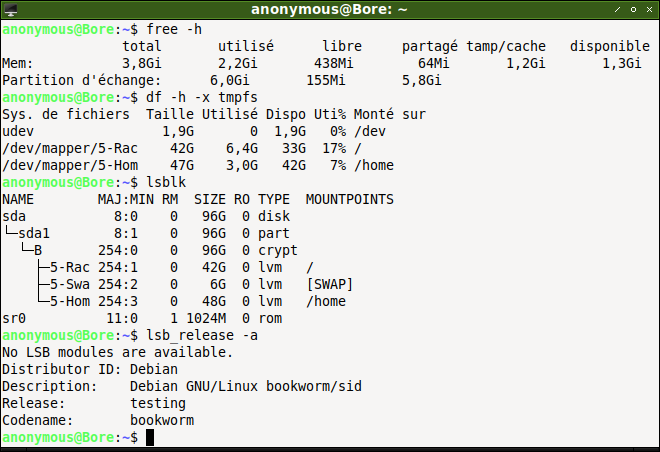
\includegraphics{terminal-final.png}
	\caption{La configuration finale obtenue}
\end{figure}

\section{Ajout d'une interface de connexion plus conviviale.}
Une fois le système posé, je vais quand même le rendre plus convivial en ajoutant une interface graphique à la fois simple d'utilisation et d'installation, je choisis xfce et j'effectue cette installation depuis le compte utilisateur via la commande \texttt{sudo}~:

\noindent \rule{\linewidth}{0.5pt}
\begin{verbatim}
sudo apt update
sudo apt install task-xfce-desktop task-french task-french-desktop
\end{verbatim}
\rule{\linewidth}{0.5pt}

Pour ma part j'ai opté pour une installation paquet par paquet en fonction de mes besoins plutôt qu'une installation par profil.
\begin{figure}
	\centering
	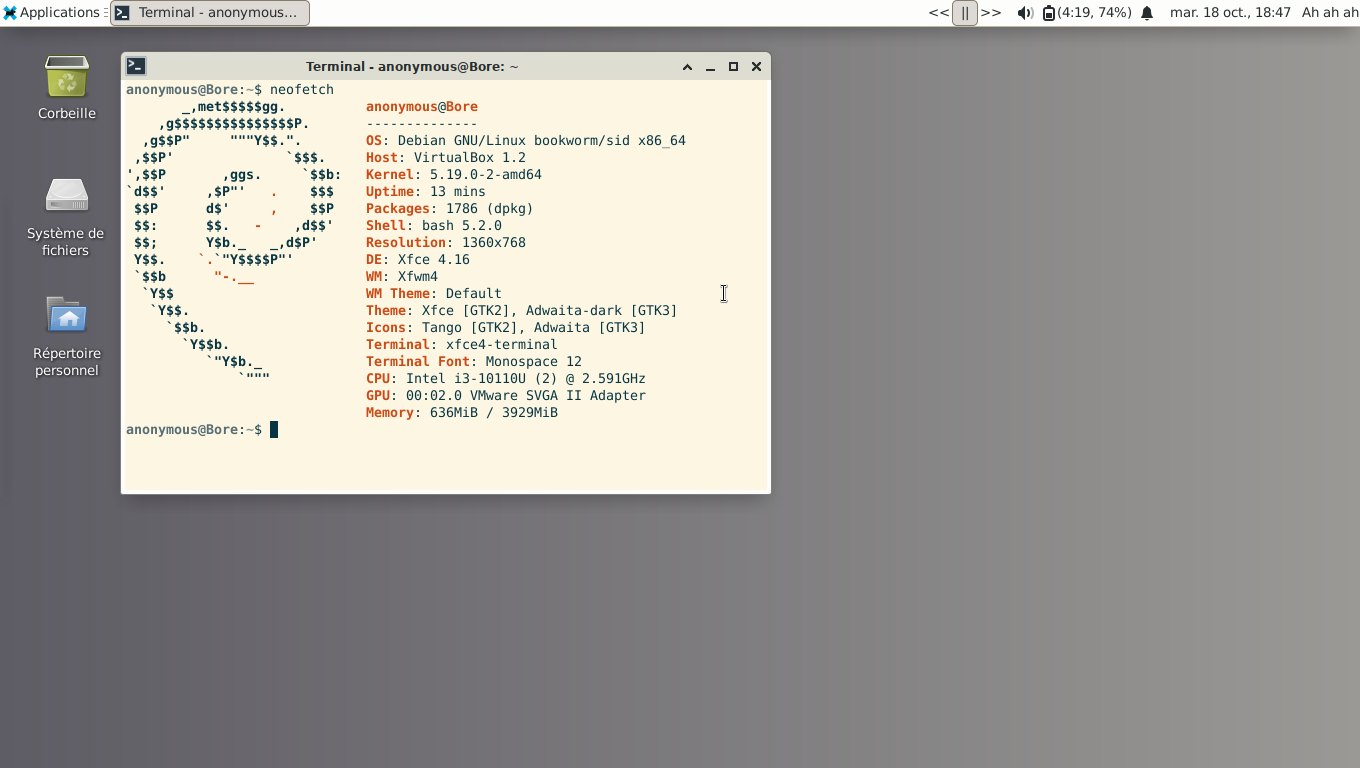
\includegraphics{xfce-desktop.png}
	\caption{La configuration finale obtenue}
\end{figure}

\section{Ajout de programmes additionnels}
Dans debian il est possible d'ajouter par défaut des programmes soit en ligne de commande, voir par exemple la section \ref{subsec-install-progs-linux} mais on peut aussi les installer via l'interface graphique dédiée nommée \texttt{synaptic} ou \texttt{kynaptic} pour ceux d'entre vous ayant installé l'interface graphique KDE.

\chapter{Cas d'une installation en uefi/secure boot} \label{sec-uefi-machine}

\texttt{/dev/sda} en table de partition gpt,
\begin{verbatim}
/dev/sda1 64M type efi
/dev/sda2 Le reste type ext4
\end{verbatim}

\begin{verbatim}
mkfs.fat -F32 /dev/sda1
cryptsetup ... /dev/sda2
\end{verbatim}

\begin{verbatim}
apt install linux-image-amd64 ... grub-efi-amd64 ...
\end{verbatim}

\begin{verbatim}
grub-install --target=x86_64-efi --bootloader-id=debian \ 
--efi-directory=/boot/efi /dev/sda
  --removable --uefi-secure boot % pas obligatoires mais utiles \
  % si disque externe
\end{verbatim}

\chapter{Compléments}
\section{Installer des programmes sous linux} \label{subsec-install-progs-linux}
L'installation de programmes sous Linux s'effectue par 3 méthodes en simplifiant, les futurs paragraphes vont les présenter succinctement.

\paragraph{La méthode usuelle~: par les paquets.}
La première consiste à utiliser un programme d'installation de paquets listés dans des dépôts, c'est l'installation la plus répandue. Chaque famille de distributions utilise un programme --~ou plusieurs~-- dédié à la gestion des paquets. Cette méthode est le plus souvent recommandée pour des raisons de sécurité~: les équipes de maintenance des paquets sont des cercles de confiance forte entre personnes qui se connaissent et reconnaissent les mérites des personnes qui les entourent, aussi devenir un membre de ses équipes n'est pas ouvert à tous.
\begin{itemize}
	\item \texttt{apt, apt-get, dpkg, dpkg-reconfigure} pour la famille debian (debian, antix, *buntu, kali, tails, mxlinux, \ldots)
	\item \texttt{yum, dnf} pour la famille des redhat, fedora, centos \ldots
	\item \texttt{pacman} pour la famille archlinux et dérivées (archlinux, artix, manjaro, parabola, hyperbola, \ldots)
	\item \texttt{pkgtool} pour la famille slackware
	\item \texttt{xbps*} pour la famille voidlinux
	\item et tant d'autres \ldots
\end{itemize}

\paragraph{Les binaires.}
La seconde plus dangereuse consiste à récupérer sur une source extérieure, typiquement un site web, le programme ou binaire prêt à l'emploi, souvent directement dans une archive. Cela est parfois nécessaire lorsqu'un programme disponible dans les dépôts est trop obsolète pour l'usage actuel ou bien que ce programme n'existe pas dans les dépôts. Cela peut prendre deux formes distinctes --~je me place dans le cas d'une distribution debian qui est l'objet de cette documentation~:
\begin{itemize}
	\item le téléchargement du binaire tel quel, j'ai pour habitude de placer de tels binaires dans le dossier \texttt{/opt} du système et de créer un lien symbolique du fichier dans \texttt{/usr/local/bin} pour que ce soit plus propre,
	\item le téléchargement d'un paquet prêt pour la distribution qui s'installer manuellement exemple, \newline
	\texttt{dpkg -i chemin/le-paquet.deb} pour debian, \newline
	ou \texttt{pacman -U chemin/le-paquet.tar.zst} pour archlinux
\end{itemize}

\paragraph{Les sources.}
La troisième pour les personnes ayant du temps ou une machine puissante consiste à installer depuis la source du logiciel, c'est le mode de fonctionnement par défaut de distributions telles que la célèbre gentoo ou l'ultime LFS. Notez que des distributions telles qu'Archlinux et tous ses clones le permettent aussi via les logiciels disponibles dans leur dépôt AUR (\emph{Arch User Repository\/}) qui liste les paquets non-maintenus par l'équipe officielle d'Archlinux mais par des développeurs contributeurs.

\section{Les versions de debian.}
\paragraph{Nommage et fréquence.}
La distribution debian a un fonctionnement spécifique qui change d'autres distributions, par exemple d'archlinux qui est de type \emph{rolling release\/} c'est-à-dire que vous l'installez à une date précise et qu'elle évolue continuellement sans changer de version à partir de ce moment-là, les paquets et le système évoluant continuellement.

Debian a un fonctionnement différent de celui d'autres distributions. 
Les différentes versions de debian sont numérotées et utilisent comme nom de code un des personnages du film d'animation \texttt{Toy Story\/}\footnote{La distribution \emph{devuan\/} dérivée directe de debian utilise quant à elle le nom des étoiles naines du système solaire tout en ayant une logique de nommage suivant le même schéma que debian.\newline
Plus d'infos ici~: \url{https://fr.wikipedia.org/wiki/Devuan}}. 
La version actuelle --~je dirai donc la version N~-- est \emph{bullseye\/}. 
Cette version est aussi désignée sous le nom de \emph{stable\/}.

Les versions stables sortent plus ou moins tous les deux ans, un an avant la sortie officielle d'une distribution stable, les paquets de la version de développement sont gelés, n'évoluant plus en versions sauf cas particulier, pour que la chasse aux \emph{bugs\/} et autres failles soit priorisée.

\paragraph{Future version et version expérimentale.}
Cette version sera suivie de la prochaine, la N+1, nommée \emph{bookworm\/} lorsqu'elle sera officiellement sortie, mais qui est aussi désignée par le nom \emph{testing\/}, où les paquets sont suffisamment stables pour que les bugs soient mineurs et qui seront considérés suffisamment mâtures pour le jour de la sortie, l'effort des développeurs étant alors de finaliser les dépendances\footnote{paquets nécessaires au fonctionnement du logiciel.} et corriger bugs et failles de sécurité.

Il existe également les paquets encore instables de la version N+2 ou \emph{sid}\footnote{Sid étant le petit garçon du film d'animation qui casse toujours ses jouets. Dans la distribution \emph{devuan} Sid=Ceres la seule planète naine de la ceinture d'astéroïdes principale.}, dont le nom ne change jamais, valant toujours Sid. 
Cette distribution est parfois confondue avec \emph{experimental\/}. 
Selon certaines sources, sid est aussi l'acronyme de \emph{Still In Developpement}.

À noter que tous les deux ans, pendant environ 1 an, les paquets de cette version évoluent beaucoup pour corriger les \emph{bugs\/} sans changer de version, puisque ces paquets sont sur le point de passer dans la distribution dite stable.

\paragraph{Anciennes versions.}
Les anciennes versions conservent leur nom de code. 
Par exemple la version actuelle en octobre 2022 moment où j'écris ces lignes est \emph{bullseye}, c'est-à-dire debian~11 mais la version 10 est encore opérationnelle et supportée, sous son nom de distribution~: \emph{buster} ou sous son autre nom \emph{old-stable}, les versions des logiciels n'évolue plus dans cette ancienne version, ou bien à la marge, mais tous les paquets reçoivent des correctifs de sécurité pour combler les failles découvertes.

La version 9 de debian, nom de code \emph{stretch\/} ou encore \emph{old-old-stable\/} se voit encore mise à jour pour les paquets essentiels du système et non les applications courantes, c'est à dire les mises-à-jour de sécurité comblant les failles. 
Par paquets essentiels s'entendent souvent ceux de l'adn de la distribution debian qui est initialement plutôt orientée serveur.

\section{Les archives de sources.}
La configuration des lignes du fichier \texttt{/etc/apt/sources.list\/} obéit à une syntaxe précise~:
\begin{verbatim}
type		url	distribution		archives
\end{verbatim}
Le type peut au choix être \texttt{deb} pour les paquets prêts à l'emploi ou \texttt{deb-scr} pour les paquets de sources logicielles, l'\texttt{url} est l'adresse où se trouvent les paquets, il existe plusieurs serveurs dans le monde, autant choisir celui qui est le plus proche de chez soi sachant que tous sont synchronisés entre eux, \texttt{distribution} est soit le nom de code de la distribution, soit certains noms spécifiques tels que \texttt{\$distribution-security} ou encore \texttt{\$distribution-backports} pour les paquets la future version de debian compatibles et compilés pour l'actuelle.

Enfin le ou les derniers paramètres de la ligne peuvent être composé d'archives, sortes de catégories de logiciels~:
\begin{itemize}
	\item \texttt{main}~: paquets de logiciels totalement libres au sens logiciel libre,
	\item \texttt{contrib}~: s'ajoute après \texttt{main} paquets de logiciels libres mais pouvant inclure des librairies externes non-libres,
	\item \texttt{non-free}~: s'ajoute après les deux précédentes paquets de logiciels non-libres
\end{itemize}
C'est souvent dans les archives \texttt{non-free} que se trouvent les firmwares propriétaires pour certains pilotes matériels.

\chapter{Notices légales.}
Ce document a été réalisé avec les logiciels \TeX{}Maker et mousepad et le moteur \texttt{pdflatex}. 
Les captures d'écran ont été réalisées avec le logiciel \texttt{xfce4-screenshooter} modifiées le cas échéant par le logiciel \texttt{kolourpaint}.

Le document a été réalisé à plus de 90\%{} dans l'environnement virtuel qui a été installé via les commandes documentées dans cet article.

\vspace{2cm}

\renewcommand{\baselinestretch}{1}
\setlength{\parskip}{0em}
\tableofcontents

\end{document}